\documentclass[aspectratio=169]{beamer}

\usetheme{Warsaw}
\usecolortheme{default}

\usepackage[T1]{fontenc}
\usepackage[utf8]{inputenc}
\usepackage{lmodern}
\usepackage{graphicx}
\usepackage{booktabs}
\usepackage{amsmath}
\usepackage{amssymb}
\usepackage{xcolor}
\usepackage{tikz}
\usetikzlibrary{shapes.geometric, arrows.meta, positioning, calc}

\graphicspath{{../report/figures/}}

\definecolor{PUT-blue}{RGB}{0,84,147}
\definecolor{PUT-dark}{RGB}{0,45,85}

\setbeamercolor{palette primary}{bg=PUT-blue,fg=white}
\setbeamercolor{palette secondary}{bg=PUT-dark,fg=white}
\setbeamercolor{palette tertiary}{bg=PUT-blue,fg=white}
\setbeamercolor{structure}{fg=PUT-blue}
\setbeamertemplate{headline}{}
\setbeamertemplate{navigation symbols}{}

\setbeamerfont{title}{size=\LARGE}
\setbeamerfont{frametitle}{size=\Large}

\title{Maritime Safety Multi-Agent Simulation}
\subtitle{Human-Factor Collision Avoidance \& SAR\\Baltic--North Sea Case Study}
\author{Pawe\l{} Pozorski, Micha\l{} Pytel}
\institute{Warsaw University of Technology}
\date{\today}

\begin{document}

\begin{frame}[plain]
    \titlepage
\end{frame}

% ═══════════════════════════════════════════════════════════════
\section{Problem}
% ═══════════════════════════════════════════════════════════════

\begin{frame}{Problem Statement}
    \begin{columns}[c]
        \begin{column}{0.65\textwidth}
            \begin{itemize}
                \item 75--96\% of maritime casualties involve \textbf{human error}
                \item COLREGs assume crews hear the warning and agree who gives way
                \item That breaks under two coupled stressors:
                \begin{itemize}
                    \item \textbf{Weather / radio:} storms cut VHF/AIS reliability
                    \item \textbf{Crew fatigue:} tired watchkeepers miss or delay CPA warnings
                \end{itemize}
                \item Many ABMs treat fatigue as a side model --- not linked to whether the manoeuvre happens
            \end{itemize}
        \end{column}
        \begin{column}{0.3\textwidth}
            \centering
            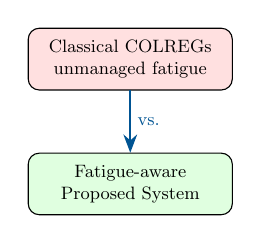
\begin{tikzpicture}[scale=0.72, transform shape, font=\small]
                \node[draw, rounded corners, fill=red!12, minimum width=3.6cm, align=center, inner sep=6pt]
                  (a) {Classical COLREGs\\unmanaged fatigue};
                \node[draw, rounded corners, fill=green!12, minimum width=3.6cm, align=center, inner sep=6pt, below=1.1cm of a]
                  (p) {Fatigue-aware\\Proposed System};
                \draw[-{Stealth}, thick, PUT-blue] (a) -- node[right]{vs.} (p);
            \end{tikzpicture}
        \end{column}
    \end{columns}
\end{frame}

% ═══════════════════════════════════════════════════════════════
\section{Hypotheses}
% ═══════════════════════════════════════════════════════════════

\begin{frame}{Research Question \& Hypotheses}
    \textbf{RQ:} Does linking fatigue management to warning reliability ($P_{\text{comms}}$) improve coordination and safety vs classical, weather-unaware practice?

    \vspace{0.5em}
    Three methods (fatigue rate $m$, weather slowdown, preparedness weight $\alpha_M$):
    \begin{itemize}
        \item \textbf{A} Classical --- $m=1.00$, no weather slowdown, $\alpha_M=2.0$
        \item \textbf{B} Shore Rest --- $m=0.82$, weather slowdown, $\alpha_M=1.3$
        \item \textbf{P} Proposed --- $m=0.65$ (smart watch), same slowdown as B, $\alpha_M=1.0$
    \end{itemize}

    \vspace{0.35em}
    Three primary hypotheses:
    \begin{itemize}
        \item \textbf{H1} --- Blind Shore: P cuts fatal rate vs A by ${\geq}20\%$
        \item \textbf{H2} --- P raises $P_{\text{prep}}$ vs A in \emph{every} scenario
        \item \textbf{H3} --- Blind Shore: P cuts collision rate vs A by ${\geq}10\%$
    \end{itemize}
\end{frame}

% ═══════════════════════════════════════════════════════════════
\section{Methodology}
% ═══════════════════════════════════════════════════════════════

\begin{frame}{Causal Safety Pipeline}
    \centering
    \resizebox{\textwidth}{!}{%
    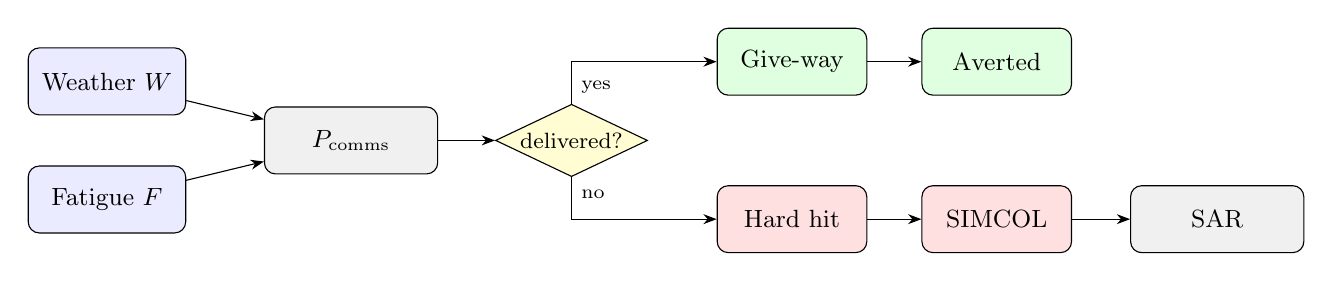
\begin{tikzpicture}[
        >=Stealth, font=\small,
        io/.style={draw, rounded corners, fill=blue!8, minimum width=2.0cm, minimum height=0.85cm, align=center},
        proc/.style={draw, rounded corners, fill=gray!12, minimum width=2.2cm, minimum height=0.85cm, align=center},
        dec/.style={draw, diamond, shape aspect=2.1, fill=yellow!18, align=center, inner sep=1pt, font=\footnotesize},
        good/.style={draw, rounded corners, fill=green!12, minimum width=1.9cm, minimum height=0.85cm, align=center},
        bad/.style={draw, rounded corners, fill=red!12, minimum width=1.9cm, minimum height=0.85cm, align=center},
    ]
        \node[io] (W) at (0,0.75) {Weather $W$};
        \node[io] (F) at (0,-0.75) {Fatigue $F$};
        \node[proc] (pc) at (3.1,0) {$P_{\text{comms}}$};
        \node[dec] (d) at (5.9,0) {delivered?};
        \node[good] (av) at (8.7,1.0) {Give-way};
        \node[good] (ok) at (11.3,1.0) {Averted};
        \node[bad] (col) at (8.7,-1.0) {Hard hit};
        \node[bad] (sim) at (11.3,-1.0) {SIMCOL};
        \node[proc] (sar) at (14.1,-1.0) {SAR};

        \draw[->] (W) -- (pc); \draw[->] (F) -- (pc); \draw[->] (pc) -- (d);
        \draw[->] (d) |- (av) node[pos=0.2, right, font=\scriptsize]{yes};
        \draw[->] (d) |- (col) node[pos=0.2, right, font=\scriptsize]{no};
        \draw[->] (av) -- (ok); \draw[->] (col) -- (sim); \draw[->] (sim) -- (sar);
    \end{tikzpicture}%
    }

    \vspace{0.5em}
    \[
      P_{\text{comms}} = \min(q_a,q_b)\,\min\big(g(F_a),\,g(F_b)\big)
    \]
\end{frame}

\begin{frame}{Scenarios \& Scale}
    \centering
    \small
    \begin{tabular}{@{}llll@{}}
        \toprule
        \textbf{Scenario} & \textbf{$N$} & \textbf{Horizon} & \textbf{Stress} \\
        \midrule
        Calm Passage & 750 & 14\,d & Fair weather; calibration \\
        Storm Corridor & 900 & ${\approx}4$\,d & Moving storm, comms $0.08$ \\
        Blind Shore & 900 & 7\,d & Patchy shore radio $0.55$ \\
        Deep Water Rescue & 500 & 7\,d & Winter SAR, slower assets \\
        \bottomrule
    \end{tabular}

    \vspace{1.8em}
    \begin{itemize}
        \item Factorial: 4 scenarios $\times$ 3 methods $\times$ 30 seeds = \textbf{360 runs}
        \item Fleets target concurrent \emph{underway} AIS scale (Baltic ${\approx}774$ moving)
        \item Stats: Mann--Whitney U, Holm over six primary contrasts, Cliff $|\delta|\ge0.2$
    \end{itemize}
\end{frame}

\begin{frame}{Primary KPIs}
    \begin{columns}[T]
        \begin{column}{0.48\textwidth}
            \begin{itemize}
                \item \texttt{fatal\_per\_1k\_hrs} --- unrecovered MOB (H1)
                \item \texttt{collision\_per\_1k\_hrs} --- rising-edge hits (H3)
                \item \texttt{mean\_p\_prep} --- crew preparedness (H2)
            \end{itemize}
            {\small
            \[
              P_{\text{prep}} = \max(0,1-\alpha_M W)\,\max(0,1-0.70\,F)
            \]}
        \end{column}
        \begin{column}{0.48\textwidth}
            \textbf{Also logged}
            \begin{itemize}
                \item Evac activation rate
                \item Survival ratio, mean TTA
                \item IWRAP $N_c$ stamp (geometry check)
            \end{itemize}
            \vspace{0.5em}
            Fatality = unrecovered person-in-water inside $\tau_{\text{mob}}$; liferaft Lost is separate.
        \end{column}
    \end{columns}
\end{frame}

\begin{frame}{Does the simulated world look right?}
    \textbf{Baseline A only} --- if this is nonsense, H1--H3 are uninterpretable.

    \vspace{0.7em}
    \begin{itemize}
        \item \textbf{Calm is not a warzone:} $0.55$ collisions / $1$k ship-hrs, inside the $0.5$--$2.0$ band we targeted
        \item \textbf{Storm actually hurts:} $3.71\times$ Calm collisions --- weather is a visible stressor
        \item \textbf{Blind carries the fatal mass:} $0.49$ fatals vs Calm $0.10$ --- that is why H1/H3 live here, not in Storm
    \end{itemize}

    \vspace{0.5em}
    \small Storm is a shared radio blackout, so methods cannot separate on fatals there.
\end{frame}

% ═══════════════════════════════════════════════════════════════
\section{GUI}
% ═══════════════════════════════════════════════════════════════

\begin{frame}{Workbench --- Map \& Playback}
    \centering
    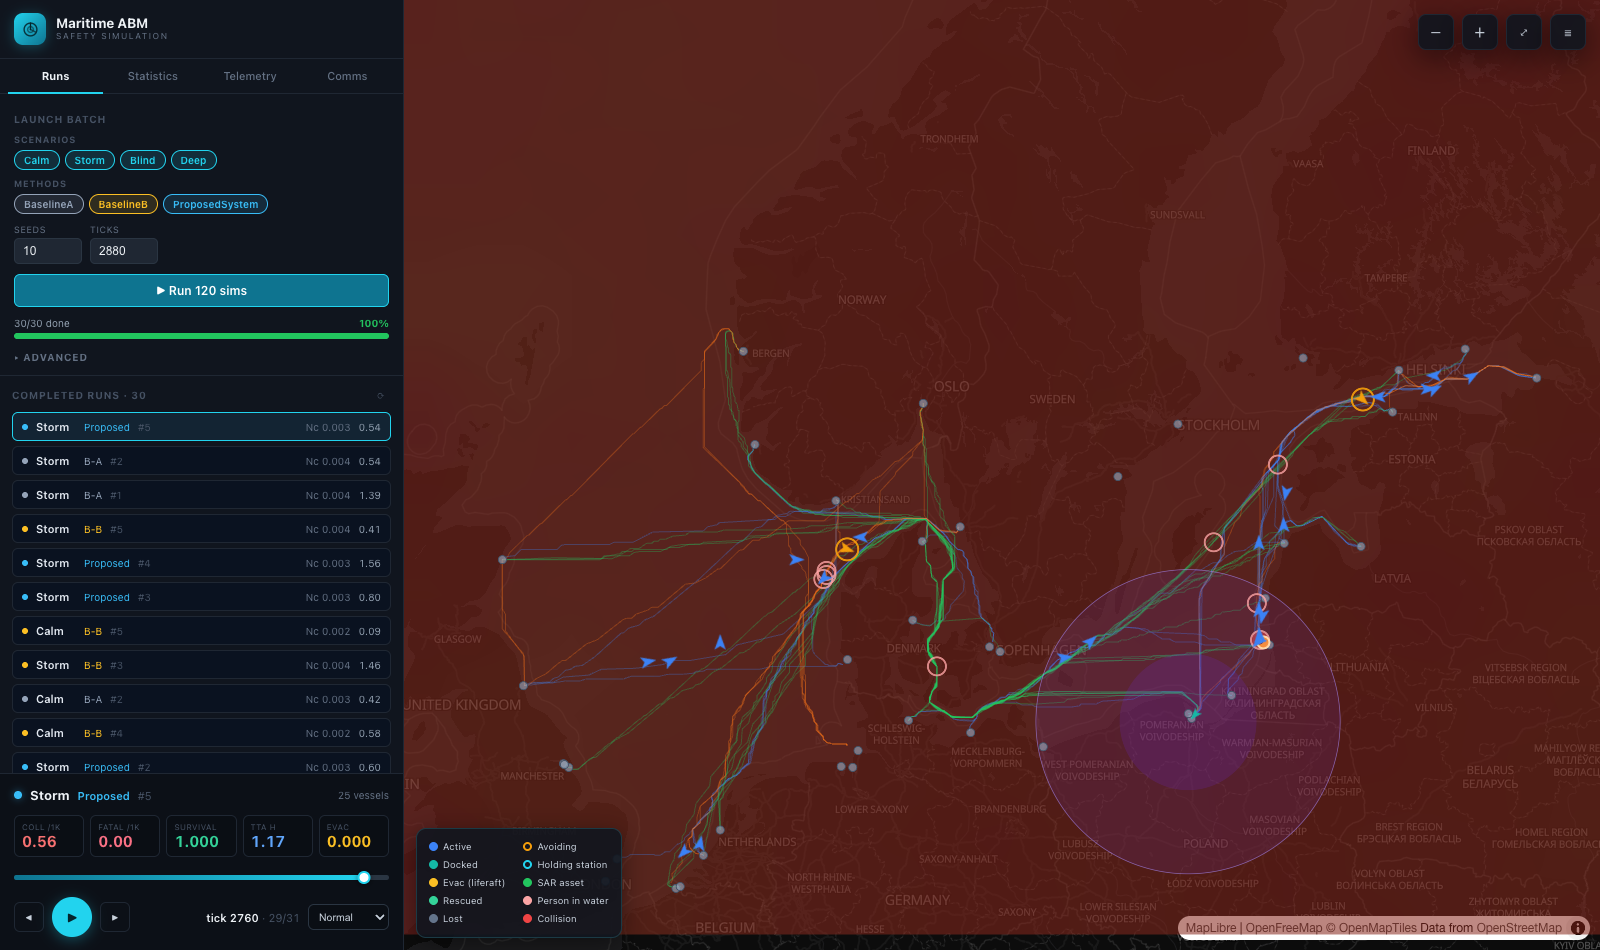
\includegraphics[width=\textwidth,height=0.78\textheight,keepaspectratio]{gui_overview.png}
\end{frame}

\begin{frame}{Workbench --- Comms Log}
    \centering
    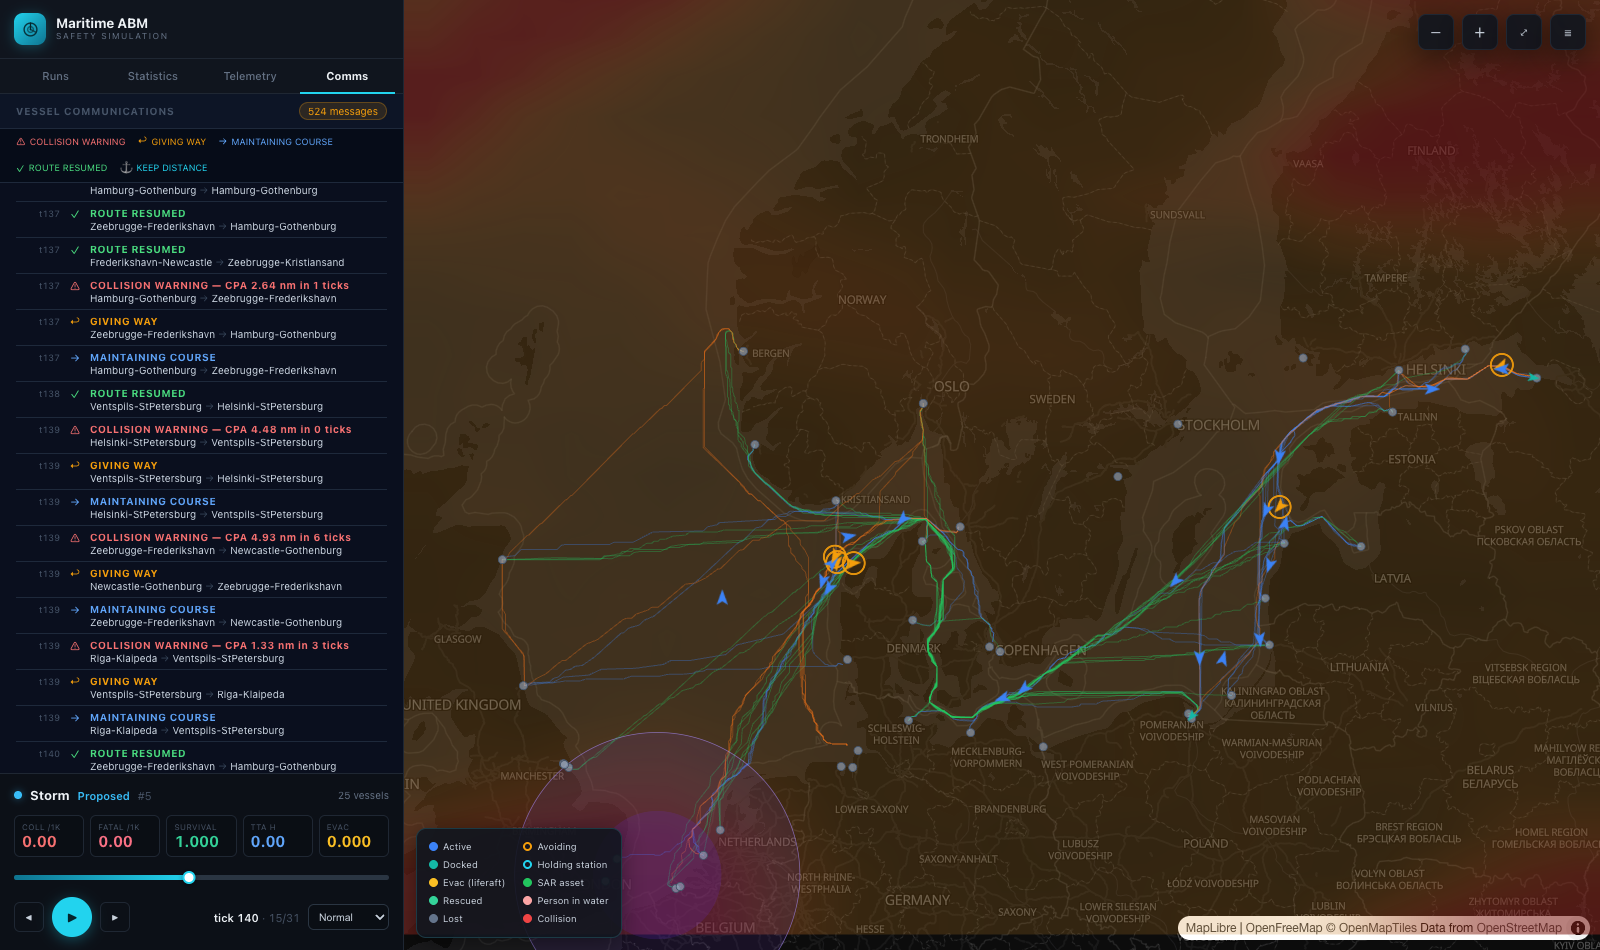
\includegraphics[width=\textwidth,height=0.78\textheight,keepaspectratio]{gui_comms.png}
\end{frame}

% ═══════════════════════════════════════════════════════════════
\section{Technical Details}
% ═══════════════════════════════════════════════════════════════

\begin{frame}{Agent Platform \& Software}
    \begin{columns}[T]
        \begin{column}{0.48\textwidth}
            \textbf{Stack}
            \begin{itemize}
                \item Engine: \textbf{Rust} + \textbf{krABMaga 0.6}
                \item Batches: Axum 0.8, Rayon, SSE
                \item Store: SQLite + JSONL tick logs
                \item UI: React 19, Vite, deck.gl~9, MapLibre
                \item Routes: \texttt{aisprocess} A$^*$ + Python fetchers
            \end{itemize}
        \end{column}
        \begin{column}{0.50\textwidth}
            \textbf{Agent computing}
            \begin{itemize}
                \item \texttt{Agent} trait: \texttt{VesselAgent}, \texttt{PostTickAgent}
                \item Schedule: vessels order 200, post-tick 1000
                \item SAR / MOB / PIW: stepped \emph{inside} post-tick (not scheduled)
                \item No FIPA/ACL --- typed in-sim \texttt{MsgKind} log
                \item COLREGs dialogue, \texttt{PostTick}-mediated, lossy $P_{\text{comms}}$
            \end{itemize}
        \end{column}
    \end{columns}
\end{frame}

\begin{frame}{Project Structure}
    \begin{columns}[T]
        \begin{column}{0.48\textwidth}
            \textbf{Engine} (\texttt{crates/simulation/})
            \begin{itemize}
                \item \texttt{vessel.rs} --- navigation, fatigue, FSM
                \item \texttt{state.rs} --- tick / post\_tick pipeline
                \item \texttt{comms.rs} --- CPA messages \& waypoints
                \item \texttt{simcol.rs} --- collision damage
                \item \texttt{sar.rs} --- liferaft \& MOB search
                \item \texttt{weather.rs} --- $50\times50$ hazard field
            \end{itemize}
        \end{column}
        \begin{column}{0.48\textwidth}
            \textbf{Repo}
            \begin{itemize}
                \item \texttt{crates/api/} --- Axum batches, SSE
                \item \texttt{frontend/} --- React / deck.gl workbench
                \item \texttt{data/} --- AIS routes, ports, coastline
                \item \texttt{report/} --- paper + figures
            \end{itemize}
        \end{column}
    \end{columns}
\end{frame}

\begin{frame}{Agent Types}
    \small
    \begin{tabular}{@{}p{3.1cm}p{4.2cm}p{5.2cm}@{}}
        \toprule
        \textbf{Agent} & \textbf{Role} & \textbf{Key behaviour} \\
        \midrule
        VesselAgent & Navigating ship & AIS route / avoidance WP; fatigue $F$; states Active$\to$Docked / Evac \\
        \addlinespace
        PostTickAgent & Shared physics & Weather, CPA, following, SIMCOL, KPI, fleet top-up \\
        \addlinespace
        RescueAgent & Liferaft SAR & Helo/Patrol: mobilise$\to$transit$\to$search$\to$embark \\
        \addlinespace
        MobSearchAgent & Person-in-water & Same phases without embark; per-person Koopman draws \\
        \addlinespace
        MobPerson & Casualty datum & Drift + $\tau_{\text{mob}}$ survival window \\
        \bottomrule
    \end{tabular}
\end{frame}

\begin{frame}{Macro-Tick Sequence}
    \small
    $\Delta t=5$\,min: step~1 \texttt{VesselAgent}, then shared \texttt{post\_tick} (2--13).

    \vspace{0.45em}
    \centering
    \footnotesize
    \begin{tabular}{@{}c l l@{}}
        \toprule
        \textbf{\#} & \textbf{Phase} & \textbf{What happens} \\
        \midrule
        1  & Navigate         & AIS route or avoidance waypoint \\
        2  & Weather          & Update hazard field $W$, storm cells \\
        3  & Grounding        & Snap off the land mask \\
        4  & Fatigue / speed  & Tick $F$; weather slowdown (B/P) \\
        5  & Comms log        & \texttt{ResumeRoute} when WP queue empties \\
        6  & Avoidance        & CPA pair; $P_{\text{comms}}$ injects starboard WP \\
        7  & Following        & Same-destination keep-distance \\
        8  & Collision        & SIMCOL: founder $\to$ Evac, else MOB \\
        9  & SAR              & Helo/patrol: search $\to$ embark / Lost \\
        10 & MOB              & PIW search; fatality if $\tau_{\text{mob}}$ elapses \\
        11 & Reap             & Drop Rescued / Lost \\
        12 & KPI / fleet      & Record KPIs; spawn until fleet $=N$ \\
        13 & Housekeeping     & UTC, storm track, JSONL snapshot \\
        \bottomrule
    \end{tabular}
\end{frame}

\begin{frame}{Vessel State Machine}
    \centering
    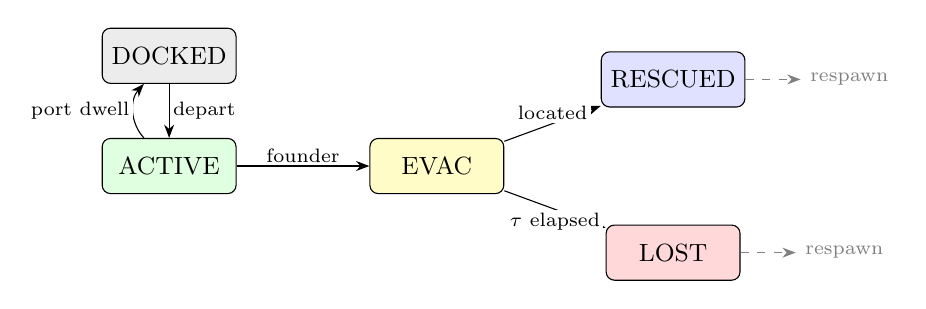
\begin{tikzpicture}[
        >=Stealth, font=\small,
        st/.style={draw, rounded corners=3pt, minimum width=1.7cm, minimum height=0.7cm, align=center},
        lab/.style={fill=white, inner sep=1.2pt, font=\scriptsize},
    ]
        \node[st, fill=gray!15]   (D) at (0,1.4)   {DOCKED};
        \node[st, fill=green!12]  (A) at (0,0)     {ACTIVE};
        \node[st, fill=yellow!22] (E) at (3.4,0)   {EVAC};
        \node[st, fill=blue!12]   (R) at (6.4,1.1) {RESCUED};
        \node[st, fill=red!15]    (L) at (6.4,-1.1){LOST};

        \draw[->] (D) -- node[lab, right]{depart} (A);
        \draw[->] (A) to[bend left=42] node[lab, left]{port dwell} (D);
        \draw[->] (A) -- node[lab, above]{founder} (E);
        \draw[->] (E) -- node[lab, above]{located} (R);
        \draw[->] (E) -- node[lab, below]{$\tau$ elapsed} (L);
        \draw[->, dashed, gray] (R.east) -- ++(0.7,0) node[right, font=\scriptsize, gray]{respawn};
        \draw[->, dashed, gray] (L.east) -- ++(0.7,0) node[right, font=\scriptsize, gray]{respawn};
    \end{tikzpicture}

    \vspace{0.6em}
    \small Foundering (SIMCOL) enters Evac; afloat overboard spawns MOB persons instead.
\end{frame}

\begin{frame}{Give-Way, MOB \& SAR}
    \begin{columns}[c,onlytextwidth]
        \begin{column}{0.31\textwidth}
            \centering
            {\scriptsize\textbf{Give-way waypoint}}
            \vspace{0.15em}

            \resizebox{\linewidth}{!}{%
            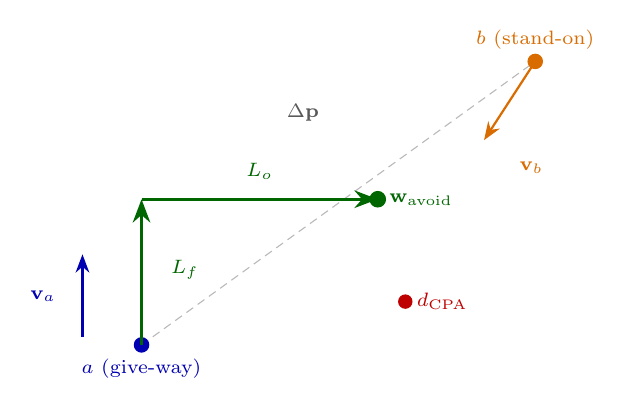
\begin{tikzpicture}[>=Stealth, font=\scriptsize,
              lab/.style={fill=white, inner sep=1pt, rounded corners=1pt}]
              \coordinate (A) at (0,0);
              \coordinate (B) at (5.0,3.6);
              \coordinate (Fwd) at (0,1.85);
              \coordinate (W) at (3.0,1.85);
              \coordinate (Cpa) at (3.35,0.55);

              \draw[densely dashed, gray!55] (A) -- (B);
              \node[lab, text=gray!70!black] at (2.05,2.95) {$\Delta\mathbf{p}$};

              \filldraw[blue!70!black] (A) circle (2.6pt);
              \node[lab, text=blue!70!black, below=4pt] at (A) {$a$ (give-way)};
              \draw[->, blue!70!black, thick] (-0.75,0.1) -- (-0.75,1.15);
              \node[lab, text=blue!70!black] at (-1.25,0.62) {$\mathbf{v}_a$};

              \filldraw[orange!85!black] (B) circle (2.6pt);
              \node[lab, text=orange!85!black, above=3pt] at (B) {$b$ (stand-on)};
              \draw[->, orange!85!black, thick] (B) -- ++(-0.65,-1.0);
              \node[lab, text=orange!85!black] at ($(B)+(-0.05,-1.35)$) {$\mathbf{v}_b$};

              \draw[->, green!40!black, very thick] (A) -- (Fwd);
              \node[lab, text=green!40!black] at (0.55,0.95) {$L_f$};
              \draw[->, green!40!black, very thick] (Fwd) -- (W);
              \node[lab, text=green!40!black] at (1.5,2.2) {$L_o$};
              \filldraw[green!40!black] (W) circle (2.8pt);
              \node[lab, text=green!40!black, right=3pt] at (W) {$\mathbf{w}_{\text{avoid}}$};

              \filldraw[red!75!black] (Cpa) circle (2.4pt);
              \node[lab, text=red!75!black, right=3pt] at (Cpa) {$d_{\text{CPA}}$};
            \end{tikzpicture}%
            }
        \end{column}
        \begin{column}{0.36\textwidth}
            \centering
            {\scriptsize\textbf{MOB search}}
            \vspace{0.15em}

            \resizebox{\linewidth}{!}{%
            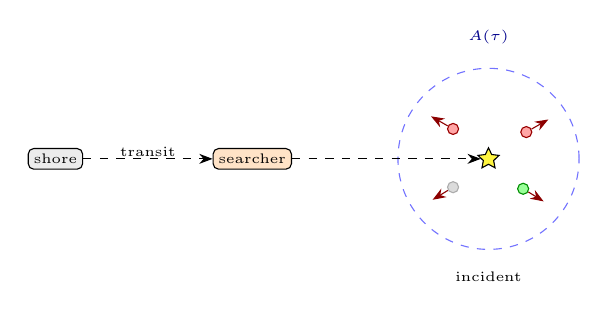
\begin{tikzpicture}[>=Stealth, font=\tiny,
              lab/.style={fill=white, inner sep=0.8pt},
              box/.style={draw, rounded corners=2pt, align=center, inner sep=2pt},
              piw/.style={circle, draw=red!60!black, fill=red!35, minimum size=4pt, inner sep=0pt},
              rec/.style={circle, draw=green!55!black, fill=green!40, minimum size=4pt, inner sep=0pt},
              lost/.style={circle, draw=gray!65, fill=gray!28, minimum size=4pt, inner sep=0pt},
            ]
              \node[box, fill=gray!15] (port) at (0,0) {shore};
              \node[box, fill=orange!22] (s) at (2.5,0) {searcher};
              \draw[->, dashed] (port) -- node[lab, above]{transit} (s);

              \coordinate (C) at (5.5,0);
              \draw[dashed, blue!55] (C) circle (1.15);
              \node[lab, text=blue!55!black] at ($(C)+(0,1.55)$) {$A(\tau)$};

              \node[star, star points=5, star point ratio=2.05, draw=black, fill=yellow!75,
                    minimum size=8pt, inner sep=0pt] (inc) at (C) {};
              \node[lab] at ($(C)+(0,-1.5)$) {incident};

              \draw[->, dashed] (s) -- (inc);

              \node[piw] (p1) at ($(C)+(-0.45,0.38)$) {};
              \draw[->, red!55!black, thin] (p1) -- ++(-0.28,0.16);
              \node[piw] (p2) at ($(C)+(0.48,0.34)$) {};
              \draw[->, red!55!black, thin] (p2) -- ++(0.28,0.16);
              \node[rec] (p3) at ($(C)+(0.44,-0.38)$) {};
              \draw[->, red!55!black, thin] (p3) -- ++(0.26,-0.16);
              \node[lost] (p4) at ($(C)+(-0.45,-0.36)$) {};
              \draw[->, red!55!black, thin] (p4) -- ++(-0.26,-0.16);
            \end{tikzpicture}%
            }

            \vspace{0.2em}
            {\tiny drifting / recovered / lost ($\tau_{\text{mob}}$)}
        \end{column}
        \begin{column}{0.31\textwidth}
            \centering
            {\scriptsize\textbf{RescuePhase}}
            \vspace{0.15em}

            \resizebox{\linewidth}{!}{%
            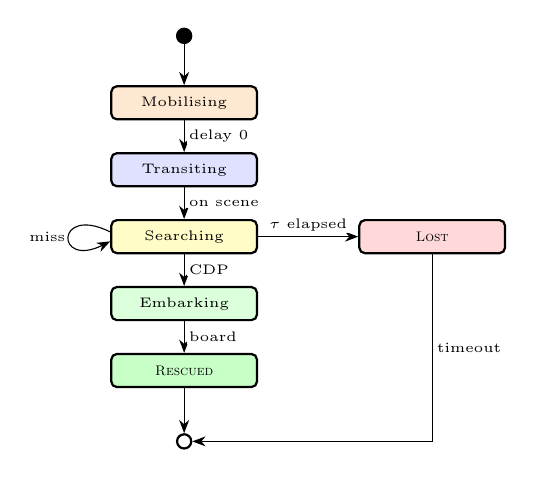
\begin{tikzpicture}[
              >=Stealth, font=\tiny,
              st/.style={draw, thick, rounded corners=2pt, minimum width=1.85cm,
                         minimum height=0.42cm, align=center, inner sep=1.5pt},
              elab/.style={font=\tiny, inner sep=0.6pt, fill=white},
              term/.style={draw, thick, circle, minimum size=0.18cm, inner sep=0pt},
            ]
              \node[term, fill=black] (start) at (0,0) {};
              \node[st, fill=orange!18] (mob) at (0,-0.85) {Mobilising};
              \node[st, fill=blue!12] (tr) at (0,-1.7) {Transiting};
              \node[st, fill=yellow!22] (se) at (0,-2.55) {Searching};
              \node[st, fill=green!14] (em) at (0,-3.4) {Embarking};
              \node[st, fill=green!22] (ok) at (0,-4.25) {\textsc{Rescued}};
              \node[term, fill=white] (end) at (0,-5.15) {};

              \node[st, fill=red!15] (lost) at (3.15,-2.55) {\textsc{Lost}};

              \draw[->] (start) -- (mob);
              \draw[->] (mob) -- (tr) node[elab, midway, right=1pt]{delay 0};
              \draw[->] (tr) -- (se) node[elab, midway, right=1pt]{on scene};
              \draw[->] (se) -- (em) node[elab, midway, right=1pt]{CDP};
              \draw[->] (em) -- (ok) node[elab, midway, right=1pt]{board};
              \draw[->] (ok) -- (end);

              \draw[->] ([yshift=0.6mm]se.west) .. controls +(-0.7,0.35) and +(-0.7,-0.35) ..
                node[elab, left=0.5pt]{miss} ([yshift=-0.6mm]se.west);

              \draw[->] (se.east) -- (lost.west)
                node[elab, midway, above=1pt]{$\tau$ elapsed};
              \draw[->] (lost.south) -- node[elab, right=1pt]{timeout}
                (lost.south |- end.east) -- (end.east);
            \end{tikzpicture}%
            }
        \end{column}
    \end{columns}
\end{frame}

\begin{frame}{Inter-Agent Communications (CPA)}
    \centering
    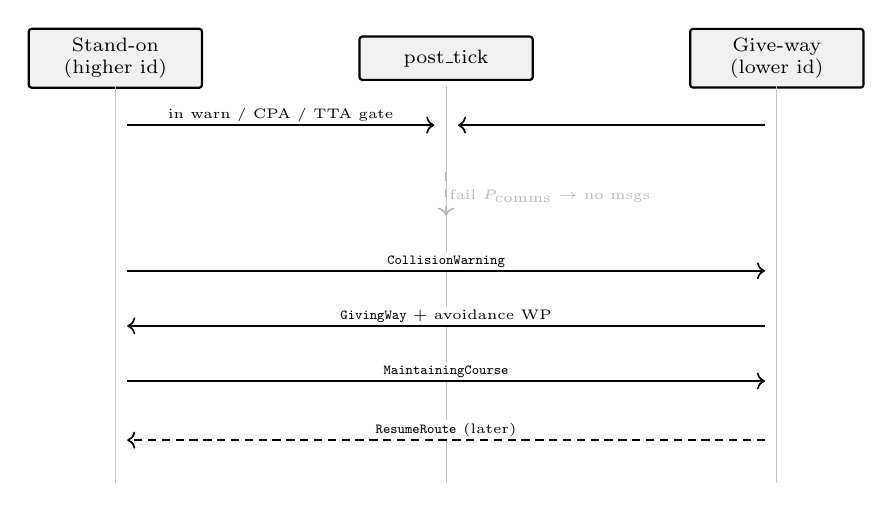
\begin{tikzpicture}[
        font=\scriptsize,
        actor/.style={draw, thick, minimum width=2.2cm, minimum height=0.55cm,
          align=center, fill=gray!12, rounded corners=1pt},
        msg/.style={->, semithick},
        nm/.style={font=\tiny, fill=white, inner sep=1pt},
    ]
        \node[actor] (so) at (0,0) {Stand-on\\(higher id)};
        \node[actor] (pt) at (4.2,0) {post\_tick};
        \node[actor] (gw) at (8.4,0) {Give-way\\(lower id)};

        \foreach \x in {0, 4.2, 8.4} {\draw[gray!45] (\x,-0.35) -- (\x,-5.4);}

        \draw[msg] (0.15,-0.85) -- (4.05,-0.85)
          node[nm, above, midway]{in warn / CPA / TTA gate};
        \draw[msg] (8.25,-0.85) -- (4.35,-0.85);

        \draw[msg, dashed, gray!55] (4.2,-1.45) -- (4.2,-2.0)
          node[nm, right, pos=0.55]{fail $P_{\text{comms}}$ $\to$ no msgs};

        \draw[msg] (0.15,-2.7) -- (8.25,-2.7)
          node[nm, above, midway]{\texttt{CollisionWarning}};
        \draw[msg] (8.25,-3.4) -- (0.15,-3.4)
          node[nm, above, midway]{\texttt{GivingWay} + avoidance WP};
        \draw[msg] (0.15,-4.1) -- (8.25,-4.1)
          node[nm, above, midway]{\texttt{MaintainingCourse}};
        \draw[msg, densely dashed] (8.25,-4.85) -- (0.15,-4.85)
          node[nm, above, midway]{\texttt{ResumeRoute} (later)};
    \end{tikzpicture}

    \vspace{0.35em}
    \small $P_{\text{comms}} = \min(q_a,q_b)\,\min(g(F_a),g(F_b))$; also \texttt{KeepDistance} on shared port approaches.
\end{frame}

% ═══════════════════════════════════════════════════════════════
\section{Results}
% ═══════════════════════════════════════════════════════════════

\begin{frame}{Hypothesis Outcomes}
    \centering
    \small
    \begin{tabular}{@{}llcc@{}}
        \toprule
        \textbf{Hyp.} & \textbf{Contrast} & \textbf{Means (A$\to$P)} & \textbf{$\delta$} \\
        \midrule
        H1 & Blind fatals & $0.486\to0.304$ (${\approx}37\%$) & $+0.53$ \\
        H2 & Calm $P_{\mathrm{prep}}$ & $0.522\to0.639$ & $-1.00$ \\
        H2 & Storm $P_{\mathrm{prep}}$ & $0.140\to0.242$ & $-0.52$ \\
        H2 & Blind $P_{\mathrm{prep}}$ & $0.401\to0.536$ & $-0.70$ \\
        H2 & Deep $P_{\mathrm{prep}}$ & $0.415\to0.543$ & $-0.77$ \\
        H3 & Blind collisions & $1.26\to1.11$ (${\approx}12\%$) & $+0.54$ \\
        \bottomrule
    \end{tabular}

    \vspace{0.7em}
    All six primary contrasts \textbf{confirmed} after Holm ($p_{\mathrm{corr}}<0.05$, $|\delta|\ge0.2$).
\end{frame}

\begin{frame}{KPI Distributions}
    \centering
    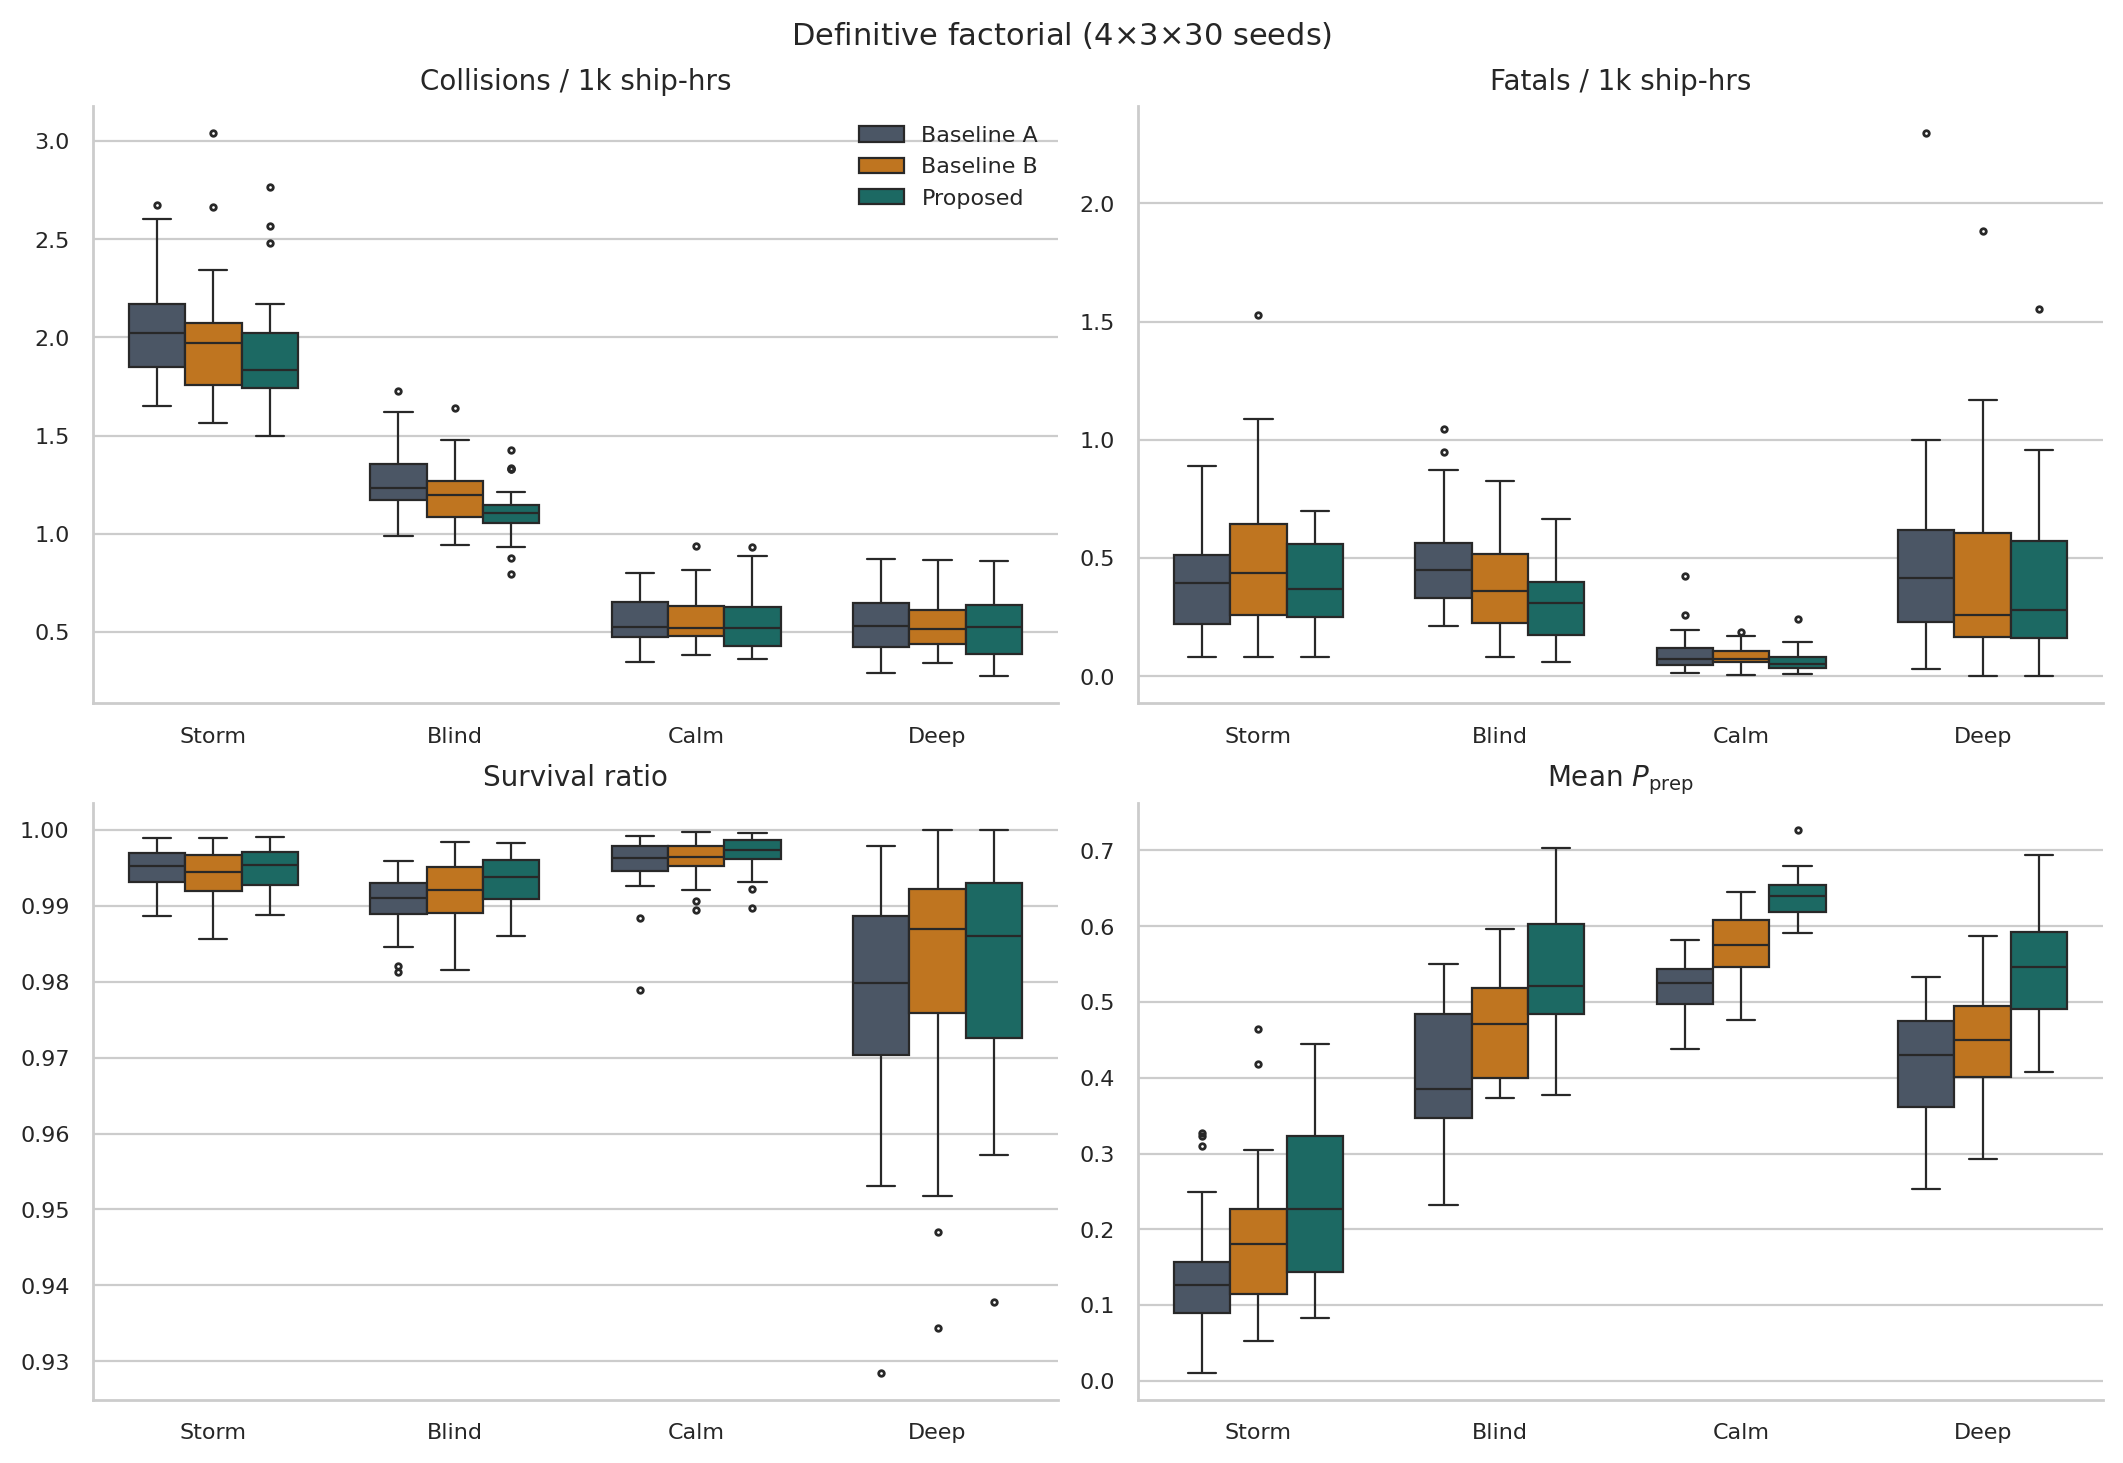
\includegraphics[width=0.82\textwidth,height=0.78\textheight,keepaspectratio]{kpi_distributions.png}
\end{frame}

\begin{frame}{Preparedness \& Storm Collisions}
    \centering
    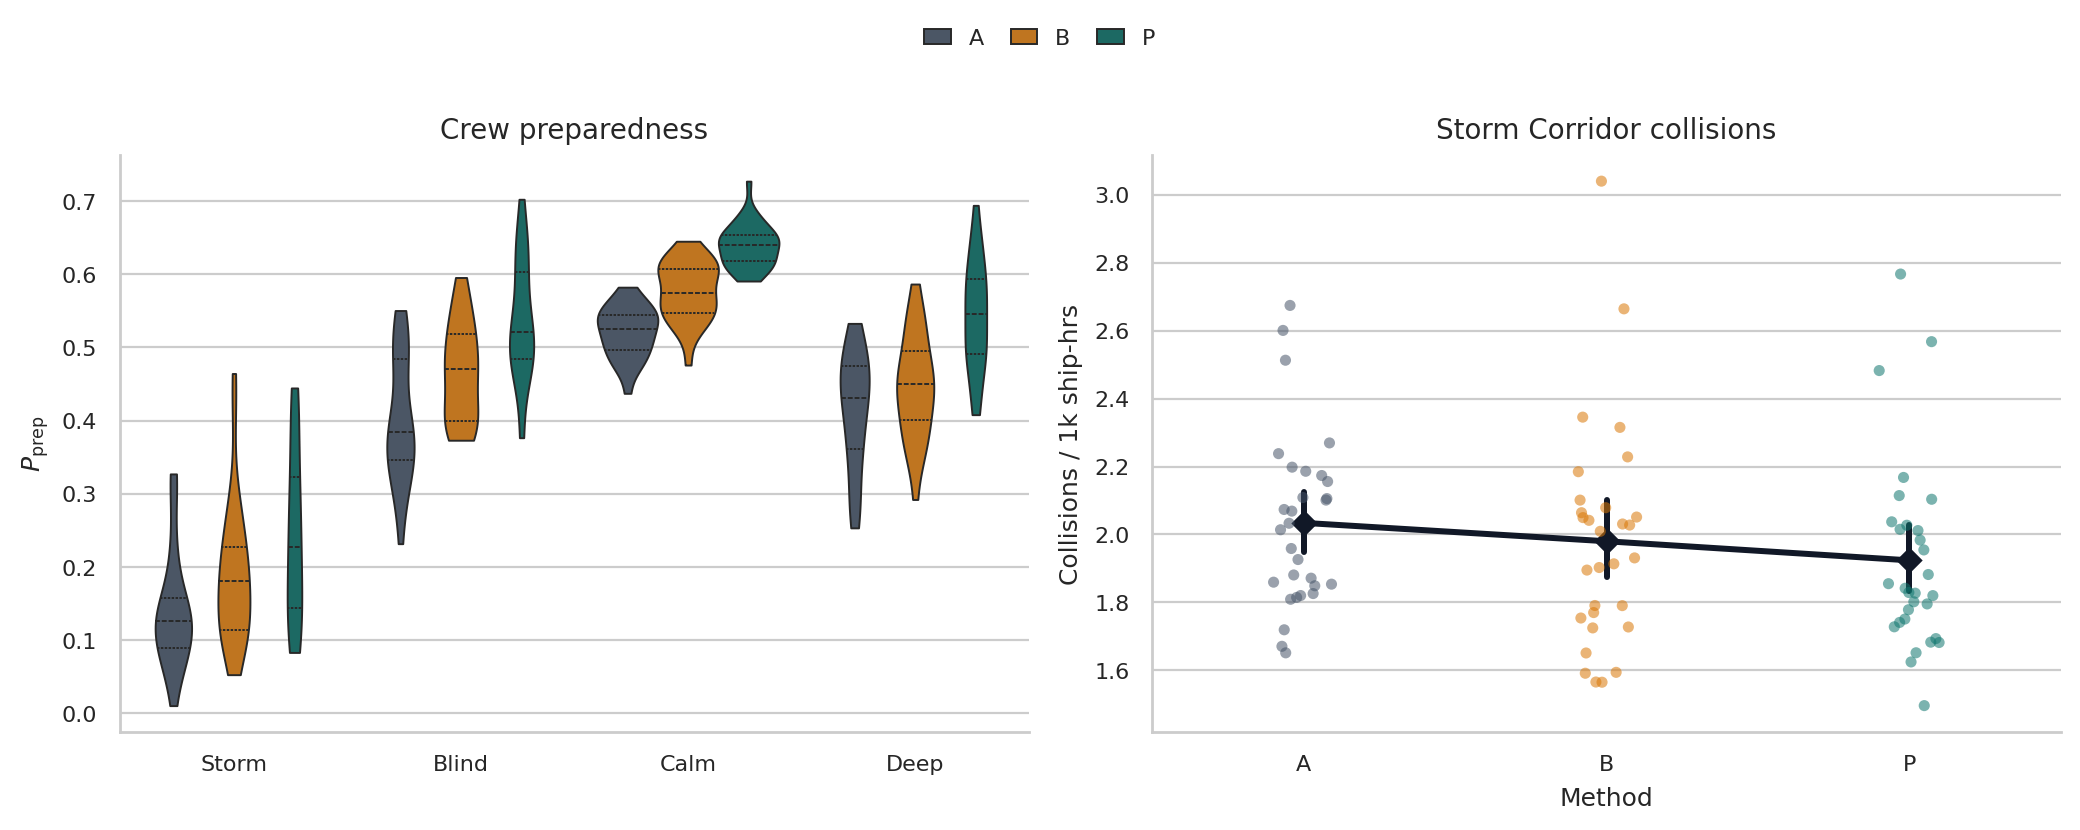
\includegraphics[width=0.85\textwidth]{preparedness_collisions.png}

    \vspace{0.3em}
    \small $P_{\mathrm{prep}}$ rises A$<$B$<$P everywhere (H2). Storm collisions fall only modestly --- shared radio blackout.
\end{frame}

\begin{frame}{Hypothesis Heatmap}
    \centering
    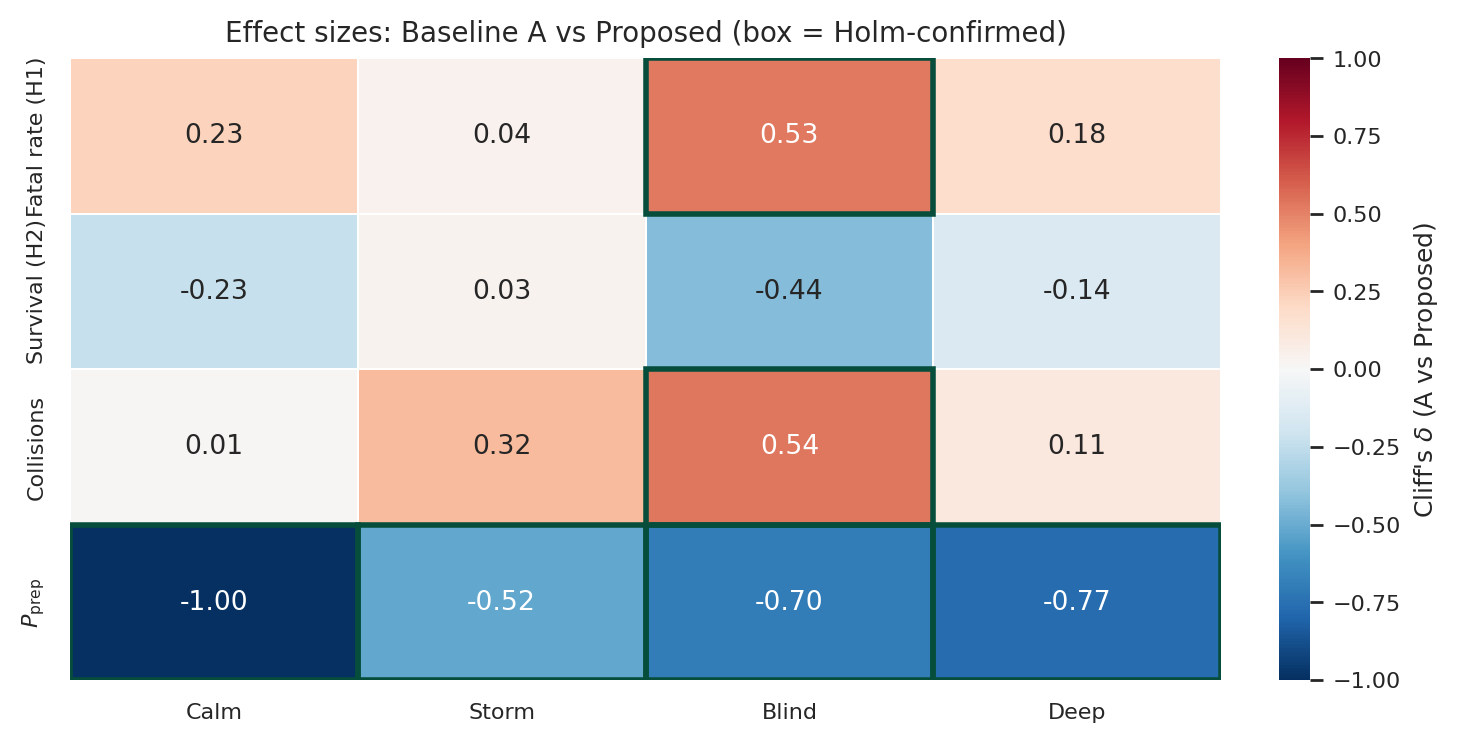
\includegraphics[width=0.72\textwidth]{hypothesis_heatmap.png}

    \vspace{0.3em}
    \small Cliff's $\delta$ for A vs P (exploratory full battery); primary H1--H3 use the six-contrast Holm set.
\end{frame}

\begin{frame}{Key Findings}
    \begin{itemize}
        \item Coupling weather + fatigue into $P_{\text{comms}}$ is an actionable lever
        \item \textbf{H1/H3 confirmed} on Blind Shore: fewer fatals (${\approx}37\%$) and collisions (${\approx}12\%$)
        \item \textbf{H2 confirmed} everywhere: Proposed raises preparedness vs Classical
        \item Storm Corridor is harsh on all methods --- shared environmental blackout
    \end{itemize}
\end{frame}

% ═══════════════════════════════════════════════════════════════
\section{Limitations}
% ═══════════════════════════════════════════════════════════════

\begin{frame}{Limitations \& Next Steps}
    \begin{columns}[T]
        \begin{column}{0.48\textwidth}
            \textbf{Limits}
            \begin{itemize}
                \item Homogeneous crew $n=20$, scalar $F$
                \item Simplified give-way (lower id)
                \item SIMCOL / Koopman surrogates
                \item No live RCC asset contention
            \end{itemize}
        \end{column}
        \begin{column}{0.48\textwidth}
            \textbf{Future}
            \begin{itemize}
                \item Heterogeneous manning / watch bills
                \item Richer COLREGs roles
                \item Contested SAR resources
                \item Transfer beyond Baltic--North Sea
            \end{itemize}
        \end{column}
    \end{columns}
\end{frame}

\begin{frame}[plain]
    \centering
    \vspace{1.8cm}
    {\Huge \textbf{Thank You!}}

    \vspace{1.2em}
    \large \textbf{Questions?}

    \vspace{1.4em}
    \normalsize
    \texttt{github.com/Michael-Pytel/maritime-abm}

    \vspace{0.8em}
    \small \{pawel.pozorski, michal.pytel2\}@pw.edu.pl
\end{frame}

\end{document}
